\documentclass{article} 
\usepackage{amsmath}
\usepackage{amssymb}
\usepackage{graphicx}
\usepackage{fancyhdr}
\usepackage{pdfpages}
\pagestyle{fancy}
\lhead{} 
\chead{} 
\lhead{\bfseries Group: SHPZKN}
\rhead{\bfseries ML Homework 8} 

\newcommand{\Lagr}{\mathcal{L}}
\newcommand{\R}{\mathbb{R}}

\begin{document}
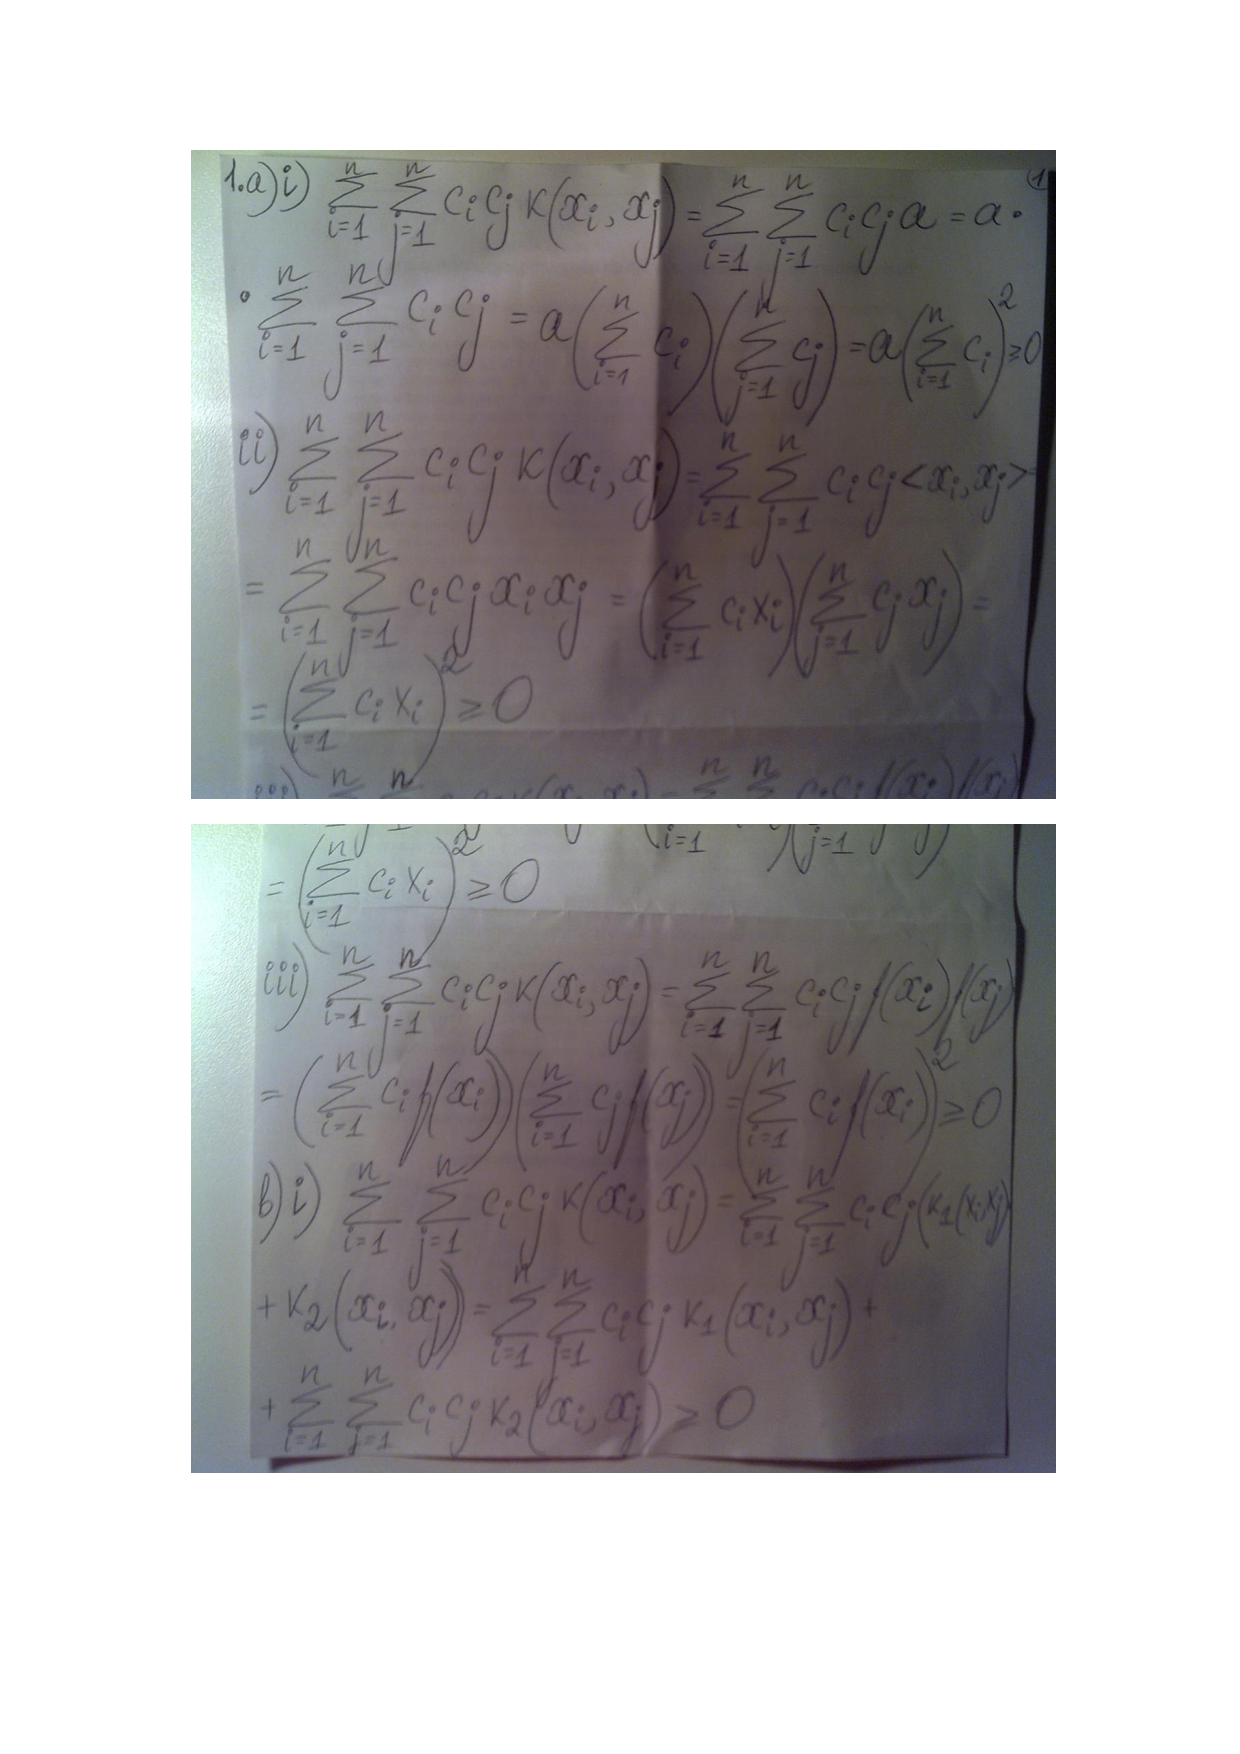
\includepdf[pages={-}]{ML8_Ex1.pdf}
\section{Problem 2}
%%% a--------------------------------------------------------------------------------------------------------------------------------
a)\\
We check if $k(x,y)=\langle \varphi(x),\varphi(y)  \rangle _\mathcal{F}$ holds:

\begin{flalign*}
\begin{split}
\langle \varphi(x),\varphi(y)  \rangle _\mathcal{F}= \langle \varphi \begin{pmatrix} x_1\\x_2 \end {pmatrix}, \varphi \begin{pmatrix} y_1\\y_2 \end {pmatrix}\rangle_\mathcal{F}&= \langle  \begin{pmatrix} x^2_1\\ \sqrt{2}x_1x_2\\ x^2_2 \end {pmatrix},\begin{pmatrix} y^2_1\\ \sqrt{2}y_1y_2\\ y^2_2 \end {pmatrix}_\mathcal{F} \\
&= x^2_1y^2_1+2x_1x_2y_1y_2+x^2_2y^2_2=(\displaystyle\sum_{i=1}^{2}x_iy_i) = \langle x,y\rangle^2 = k(x,y)
\end{split}&
\end{flalign*}
%%%% b----------------------------------------------------------------------------------------------------------------------------------
b)\\
i)
\begin{flalign*}
\begin{split}
\varphi(\mathcal{C}) = \varphi \begin{pmatrix} cos(\theta)\\ sin(\theta) \end {pmatrix} = \begin{pmatrix} cos(\theta)^2\\ \sqrt{2}cos(\theta)sin(\theta)\\ sin(\theta)^2 \end {pmatrix}\\
\end{split}&
\end{flalign*}
 for $0 \leq \theta <2\pi$\\
ii)
\begin{flalign*}
\begin{split}
\varphi(\mathcal{A}) = \varphi \begin{pmatrix} t\\ s \end {pmatrix} = \begin{pmatrix}t^2\\ \sqrt{2}ts\\ s^2 \end {pmatrix}\\
\end{split}&
\end{flalign*}
for s,t $\in \mathbb{R}$
\\
c)\\
We know that $cos(\theta)^2+sin(\theta)^2 =1$, also that $2sin(\theta)cos(\theta)=sin(2\theta)$.\\
 Now we define $\mathnormal{v}=cos(\theta)^2$ and $\mathnormal{w}=\frac{\sqrt{2}}{2}sin(2\theta)$
\begin{flalign*}
\begin{split}
 \begin{pmatrix} cos(\theta)^2\\ \sqrt{2}cos(\theta)sin(\theta)\\ sin(\theta)^2 \end {pmatrix}= \begin{pmatrix} cos(\theta)^2\\ \frac{\sqrt{2}}{2}sin(2\theta)\\1-cos(\theta)^2 \end {pmatrix}=\begin{pmatrix}\mathnormal{v}\\ \mathnormal{w}\\ 1-\mathnormal{v} \end {pmatrix}\\
\end{split}&
\end{flalign*}
\\
d)\\
It is easy to show that:
\begin{flalign*}
\begin{split}
P=\begin{pmatrix}P_x\\ P_y\\ P_z \end {pmatrix}=\begin{pmatrix}1\\ 0\\ 1 \end {pmatrix}
\notin \varphi (\mathcal{A})\\
\end{split}&
\end{flalign*}
We choose $P_x=t^2=1$, so it holds that t=1 and $P_z=s^2=1$, where follows that s=1.\\ In $\varphi (\mathcal{A})$ it should hold that $P_y=\sqrt{2}st$, but it is $\sqrt{2}st=\sqrt{2}\neq0=P_y$ instead.
\end{document}